% CVPR 2026 Paper Template; see https://github.com/cvpr-org/author-kit
% VQA-Disagree: Multi-Model Disagreement as an Annotation-Free Difficulty Signal
% DataMFM @ CVPR 2026 Workshop -- Non-archival short paper

\documentclass[10pt,twocolumn,letterpaper]{article}

%%%%%%%%% PAPER TYPE  - arXiv version (accepted at DataMFM @ CVPR 2026)
% \usepackage{cvpr}              % camera-ready (no page numbers)
% \usepackage[review]{cvpr}      % review (line numbers, anonymous)
\usepackage[pagenumbers]{cvpr}  % arXiv version: final layout with page numbers

% Standard packages
\usepackage{times}
\usepackage{graphicx}
\usepackage{amsmath}
\usepackage{amssymb}
\usepackage{booktabs}
\usepackage{multirow}
\usepackage{microtype}
\usepackage{xcolor}
\usepackage{enumitem}

% Hyperref with the colors recommended by the CVPR 2026 author-kit.
% cleveref must follow hyperref.
\definecolor{cvprblue}{rgb}{0.21,0.49,0.74}
\usepackage[pagebackref,breaklinks,colorlinks,allcolors=cvprblue]{hyperref}
\usepackage{cleveref}

%%%%%%%%% PAPER ID  - PLEASE UPDATE
\def\paperID{*****} % *** Enter the Paper ID here
\def\confName{CVPR}
\def\confYear{2026}

\newcommand{\dname}{\textsc{VQA-Disagree}}
\newcommand{\dscore}{$D$}
\newcommand{\ie}{\emph{i.e.},}
\newcommand{\eg}{\emph{e.g.},}
\newcommand{\etal}{\emph{et al.}}

\begin{document}

\title{\dname{}: Multi-Model Disagreement as an\\Annotation-Free Difficulty Signal for VQA Benchmarks\thanks{Accepted (Paper~\#29) at the DataMFM Workshop, CVPR 2026 (non-archival): \href{https://datamfm.github.io/}{\nolinkurl{datamfm.github.io}}.}}

\author{Ashwin Prakash\\
The University of Texas at Austin\\
{\tt\small ashwinprakash@utexas.edu}
}

\maketitle

% ============================================================
\begin{abstract}
Visual question answering benchmarks treat all samples as equal-weight evaluation
signal, yet in practice a large fraction are trivially easy: every
current vision-language model (VLM) answers them correctly.  Such
\emph{saturated} samples contribute almost no information when comparing models.
We propose \emph{multi-model disagreement}---the fraction of distinct answer
clusters produced by an ensemble of four architecturally diverse
VLMs---as a cheap, annotation-free proxy for sample difficulty.  Applying
this metric to 1,500 questions drawn from four public VQA benchmarks spanning
natural scenes, scene-text, charts, and real-world photographs (VQAv2,
TextVQA, ChartQA, and RealWorldQA), we find that
\textbf{5.4\%} of samples are saturated (unanimous and correct),
while \textbf{50.1\%} are genuinely hard (high-disagreement).  Qwen2-VL-72B
used as a scale-based oracle confirms a \textbf{28.3}~pp Easy--Hard
accuracy gap and an even larger \textbf{36.6}~pp Easy--Deceptive gap
(38.3\% vs.\ 1.7\%), validating disagreement as a difficulty signal.
The \emph{deceptive} subcategory---unanimous but wrong---turns out to be
the hardest stratum for the oracle, suggesting it captures shared
architectural blind spots rather than mere model-family idiosyncrasies.
We release \dname{}, a 456-sample difficulty-stratified subset on
HuggingFace Hub, intended as a more informative evaluation slice for the
multimodal community.
\end{abstract}

% ============================================================
\section{Introduction}
\label{sec:intro}

The rapid capability growth of vision-language models has created a
familiar problem in benchmark evaluation: saturation.  On established
datasets such as VQAv2~\cite{goyal2017vqav2} and
GQA~\cite{hudson2019gqa}, top-performing models already exceed 80\%
accuracy, compressing the signal available for distinguishing them.
Comprehensive evaluations confirm this trend across dozens of multimodal
tasks~\cite{fu2024mmbench}.  Yet benchmark curators rarely retire samples
once they become easy, meaning that each new paper wastes compute
evaluating questions that every VLM has already solved.

The standard remedy---collecting new, harder benchmarks---is expensive and
slow.  We argue for a complementary, automatic approach: rather than
replacing benchmarks, \emph{stratify} them by difficulty using a signal
that is already available: the \emph{disagreement} of a small ensemble of
diverse VLMs~\cite{swayamdipta2020cartography}.  When four models of
different architectures all give the same answer, that question is very
likely easy (or at worst, consistently misleading).  When they give four
different answers, the question is genuinely ambiguous or hard.  Rather
than discarding or replacing saturated benchmarks, this annotation-free
stratification automatically identifies the subset that still provides
discriminative signal.

Concretely, we define a disagreement score $D \in [0, 1]$ computed from
semantic clustering of predictions (Section~\ref{sec:method}) and use it
to assign each sample to one of four strata: \emph{Easy} ($D=0$, all
correct), \emph{Deceptive} ($D=0$, all wrong), \emph{Medium}
($D=0.25$), and \emph{Hard} ($D \geq 0.5$).  We apply this pipeline
to 1,500 samples spanning four publicly available benchmarks, validate the
strata against a Qwen2-VL-72B oracle, and release \dname{}---a 456-sample
difficulty-stratified subset---on HuggingFace Hub.

\paragraph{Contributions.}
\begin{enumerate}[leftmargin=*,topsep=2pt,itemsep=1pt]
\item A reproducible, annotation-free difficulty metric based on
  multi-model semantic disagreement (\S\ref{sec:method}).
\item An empirical characterisation of how difficulty distributes across
  four public VQA benchmarks and seven question types (\S\ref{sec:results}).
\item Validation that both high-disagreement and unanimous-but-wrong
  samples are genuinely harder, using Qwen2-VL-72B as a scale-based oracle
  on 455 items spanning all four strata (\S\ref{sec:validation}).
\item The \dname{} dataset: 456 difficulty-stratified VQA samples with
  full metadata, released publicly for community use (\S\ref{sec:conclusion}).
\end{enumerate}

% ============================================================
\section{Related Work}
\label{sec:related}

\paragraph{Benchmark saturation and renewal.}
Benchmark saturation---where top models converge near ceiling accuracy---is
now well-documented in vision-language evaluation~\cite{fu2024mmbench}.
Responses include constructing harder benchmarks and data
cartography~\cite{swayamdipta2020cartography}, which uses training dynamics
to identify \emph{easy}, \emph{ambiguous}, and \emph{hard-to-learn} samples.
Our work adapts the cartography intuition to the multimodal, inference-only
setting: we replace training dynamics with multi-model disagreement,
requiring no fine-tuning.

\paragraph{Data quality and pruning.}
Prior work on dataset pruning~\cite{sorscher2022beyond} and
quality-guided selection~\cite{gadre2024datacomp} shows that a well-chosen
subset outperforms random sampling at equal size.  We bring this lens to
VQA \emph{evaluation}: our disagreement score identifies the subset of
existing benchmarks that still provides discriminative signal.

\paragraph{VLM evaluation benchmarks.}
Recent work has exposed systematic visual shortcomings of current
VLMs~\cite{tong2024mmvp}, including failures on chart interpretation and
fine-grained visual grounding.  Our contribution is orthogonal: rather than
curating new content, we characterise difficulty within \emph{existing}
benchmarks and release a stratified slice that concentrates signal in the
Hard and Deceptive strata.

% ============================================================
\section{Method}
\label{sec:method}

\subsection{Source Datasets and Sampling}
\label{sec:datasets}

We draw samples from four publicly available VQA benchmarks chosen to span
a wide range of visual domains and question styles:
\textbf{VQAv2}~\cite{goyal2017vqav2} (general everyday scenes, 500 samples
from the validation split);
\textbf{TextVQA}~\cite{singh2019textvqa} (text recognition in natural images,
300 from the validation split);
\textbf{ChartQA}~\cite{masry2022chartqa} (chart and figure understanding,
500 from the validation split);
and \textbf{RealWorldQA}~\cite{realworldqa2024} (real-world photographs,
200 from the test set).
The total corpus is \textbf{1,500} image-question pairs.

\subsection{VLM Ensemble}
\label{sec:models}

Meaningful disagreement requires architectural diversity; a set of nearly
identical models will converge on similar errors.  We select four
open-source VLMs spanning a wide range of visual encoders and language
backbones (Table~\ref{tab:models}):
Qwen2-VL-7B-Instruct~\cite{wang2024qwen2vl} (dynamic-resolution ViT + Qwen2);
LLaVA-1.6-Mistral-7B~\cite{liu2024llava16} (CLIP ViT-L + Mistral-7B);
InternVL2-8B~\cite{chen2024internvl} (InternViT-300M + InternLM2-7B);
and MiniCPM-V~2.6~\cite{yao2024minicpmv} (SigLIP + MiniCPM-3B).
All models run at bfloat16 precision on A100-40GB GPUs with no quantisation.
Each model answers each question independently with greedy decoding
(\texttt{max\_new\_tokens=64}, \texttt{do\_sample=False}).
No brevity instruction is prepended; each model receives the raw question string
paired with the image, using its default chat template.

\begin{table}[t]
\centering
\caption{VLM ensemble used for disagreement scoring.}
\label{tab:models}
\small
\begin{tabular}{llll}
\toprule
Tag & Model & Visual enc. & LM backbone \\
\midrule
\texttt{qwen}     & Qwen2-VL-7B     & Dynamic ViT & Qwen2-7B \\
\texttt{llava}    & LLaVA-1.6-M-7B  & CLIP ViT-L  & Mistral-7B \\
\texttt{internvl} & InternVL2-8B    & InternViT-300M & InternLM2-7B \\
\texttt{minicpm}  & MiniCPM-V~2.6   & SigLIP      & MiniCPM-3B \\
\bottomrule
\end{tabular}
\end{table}

\subsection{Disagreement Score}
\label{sec:disagree}

Given four predictions $p_1, p_2, p_3, p_4$ for a sample, we compute
the disagreement score $D$ as follows.

\paragraph{Step 1: normalisation.}
Each prediction is lowercased, punctuation-stripped, and article-removed
following the standard VQA normalisation~\cite{antol2015vqa}.

\paragraph{Step 2: semantic clustering.}
Normalised predictions are first grouped by exact string match.
We then merge groups whose representative sentence-BERT
embeddings~\cite{reimers2019sbert} exceed cosine similarity $\geq 0.8$,
handling semantically equivalent paraphrases (\eg ``automobile'' and ``car'').
A threshold sweep at $\{0.70, 0.85, 0.90\}$ preserves 84.8\% of stratum
labels at $\pm0.05$ from our 0.80 default, confirming label stability.

\paragraph{Step 3: disagreement score.}
Let $k^* = \max_j |C_j|$ be the size of the largest prediction cluster.
\begin{equation}
  D = 1 - \frac{k^*}{4}.
  \label{eq:disagree}
\end{equation}
$D=0$ means all four models agree; $D=0.75$ means all four give different
answers.

\paragraph{Stratum assignment.}
Each sample is additionally scored for correctness against the ground truth
using VQA soft accuracy~\cite{antol2015vqa} (for VQAv2 and TextVQA, both of
which provide multiple human annotations) or normalised exact match (for ChartQA
and RealWorldQA), yielding four strata:
\begin{itemize}[leftmargin=*,topsep=2pt,itemsep=0pt]
\item \textbf{Easy} ($D=0$, all correct): saturated; minimal benchmark value.
\item \textbf{Deceptive} ($D=0$, all wrong): unanimous systematic error;
  reveals architectural blind spots.
\item \textbf{Medium} ($D=0.25$, 3-of-4 agree): contested; one model diverges.
\item \textbf{Hard} ($D \geq 0.5$, no 3+ consensus): high information;
  models genuinely disagree.
\end{itemize}

\subsection{Scale-Based Oracle Validation}
\label{sec:oracle}

To confirm that high-disagreement and unanimous-but-wrong strata reflect genuine
task difficulty---rather than idiosyncratic failure modes of the four 7B-scale
ensemble members---we run Qwen2-VL-72B-Instruct~\cite{wang2024qwen2vl}
($\approx$10$\times$ larger) on 455 items: 81 Easy, 100 Medium, 100 Hard,
and all 174 Deceptive samples.
Using a same-family model at much larger scale is a \emph{stronger} argument
than cross-family agreement: if the Hard stratum remains harder for a 72B model
sharing pre-training lineage with one ensemble member, the difficulty is
structural rather than a product of architectural disagreement.
The 72B model is loaded with 4-bit NF4 quantisation~\cite{dettmers2023qlora}
on an A100-80GB GPU.

% ============================================================
\section{Results}
\label{sec:results}

\begin{figure}[t]
  \centering
  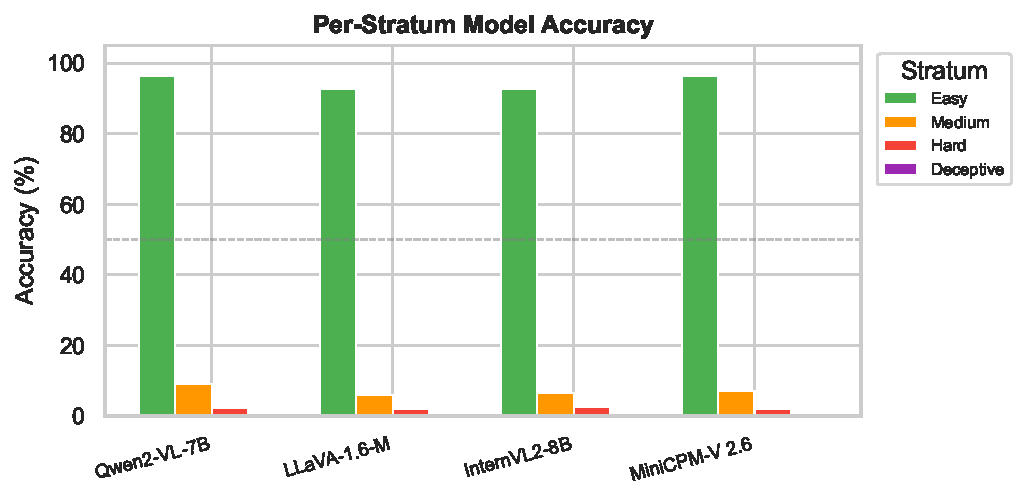
\includegraphics[width=\linewidth]{figures/fig1_teaser.pdf}
  \caption{%
    \textbf{Per-stratum model accuracy.}
    Easy samples are answered correctly by nearly all models ($>$92\%);
    Hard samples see accuracy collapse to 2--3\%, confirming disagreement
    as a difficulty signal.}
  \label{fig:teaser}
\end{figure}

\subsection{Stratum Distribution}
\label{sec:distribution}

\begin{table}[t]
\centering
\caption{Per-source-dataset stratum statistics.}
\label{tab:datasets}
\small
\begin{tabular}{lrcccc}
\toprule
Dataset & N & Easy\% & Medium\% & Hard\% & Deceptive\% \\
\midrule
ChartQA & 500 & 0.0 & 27.2 & 68.6 & 4.2 \\
RealWorldQA & 200 & 40.5 & 32.5 & 21.0 & 6.0 \\
TextVQA & 300 & 0.0 & 43.0 & 56.0 & 1.0 \\
VQAv2 & 500 & 0.0 & 32.6 & 39.8 & 27.6 \\
\bottomrule
\end{tabular}
\end{table}

\begin{figure}[t]
  \centering
  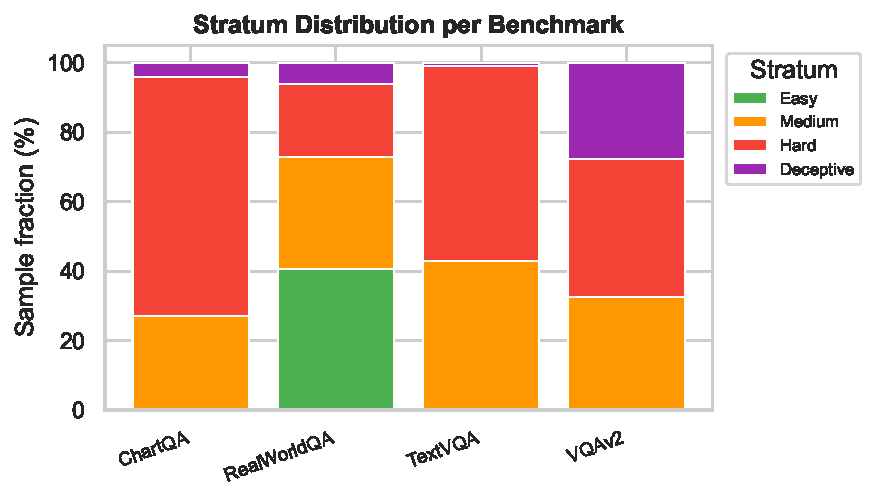
\includegraphics[width=\linewidth]{figures/fig2_stacked_distribution.pdf}
  \caption{%
    \textbf{Stratum distribution per benchmark.}
    RealWorldQA has the highest Easy fraction (40.5\%); ChartQA and TextVQA
    are dominated by Hard samples.  VQAv2's large Deceptive fraction (27.6\%)
    reflects systematic answer-format mismatch between model outputs and the
    short-form annotation convention.}
  \label{fig:distribution}
\end{figure}

\Cref{tab:datasets} reports the fraction of each stratum per source dataset.
Across the full corpus, \textbf{5.4\%} of samples fall in the Easy stratum
(\ie they have been effectively ``solved'' by all four VLMs).
The saturated fraction varies substantially across datasets: RealWorldQA has
the highest Easy fraction (\textbf{40.5\%}), suggesting that presence/absence
and coarse attribute questions in real-world photographs are largely mastered
at 7B scale.  In contrast, VQAv2, TextVQA, and ChartQA have \textbf{0\%} Easy
samples, indicating that none of the 1,300 probed questions on these three benchmarks
were answered correctly by all four models unanimously---even for VQAv2, where
models systematically generate verbose answers that fail normalized exact match
against the expected short-form human annotations.

The Deceptive stratum accounts for \textbf{11.6\%} of all samples---of which
\textbf{27.6\%} of VQAv2 samples fall in this stratum, by far the highest rate.
Manual inspection of 25 random Deceptive samples reveals two causes:
\textbf{(a) answer-format mismatch}, where models produce verbose, semantically
correct responses (\eg ``Yes, there is a red sandal in the image.'') that
fail the short-form VQAv2 convention (``yes''); and \textbf{(b) genuine shared
visual errors} such as systematic miscounts or fine-grained colour confusions
across all four architectures.  Case (a) dominates in VQAv2; the oracle
analysis in \Cref{sec:validation} shows case (b) dominates elsewhere.

\Cref{fig:distribution} shows the stacked stratum distribution per dataset.
ChartQA has the highest Hard fraction (\textbf{68.6\%}), confirming that
chart-reading requires specialised visual reasoning not yet solved at 7B
scale.

\subsection{Per-Model Accuracy per Stratum}
\label{sec:accuracy}

\begin{table}[t]
\centering
\caption{Accuracy (\%) per model on each stratum.}
\label{tab:accuracy}
\small
\begin{tabular}{lcccc}
\toprule
Model & Easy & Medium & Hard & Deceptive \\
\midrule
Qwen2-VL-7B & 96.3 & 9.1 & 2.3 & 0.0 \\
LLaVA-1.6-M & 92.6 & 6.1 & 2.0 & 0.0 \\
InternVL2-8B & 92.6 & 6.5 & 2.7 & 0.0 \\
MiniCPM-V 2.6 & 96.3 & 7.1 & 2.0 & 0.0 \\
\bottomrule
\end{tabular}
\end{table}

\Cref{tab:accuracy} reports individual model accuracy on each stratum.
Easy accuracy ranges from 92.6\% to 96.3\% across models---near-perfect but
below 100\%, as sentence-BERT-based clustering can group semantically similar
predictions that still differ from the normalized ground-truth string.  On
Hard samples, per-model accuracy collapses to \textbf{2.0\%--2.7\%}, with
InternVL2-8B performing marginally better than the other ensemble members.
The Deceptive stratum yields 0\% accuracy for every model---by
construction, since Deceptive requires all four predictions to cluster together
while failing the ground truth.

\Cref{fig:teaser} visualises these results across models and strata.

\subsection{Qwen2-VL-72B Oracle Validation}
\label{sec:validation}

\begin{figure}[t]
  \centering
  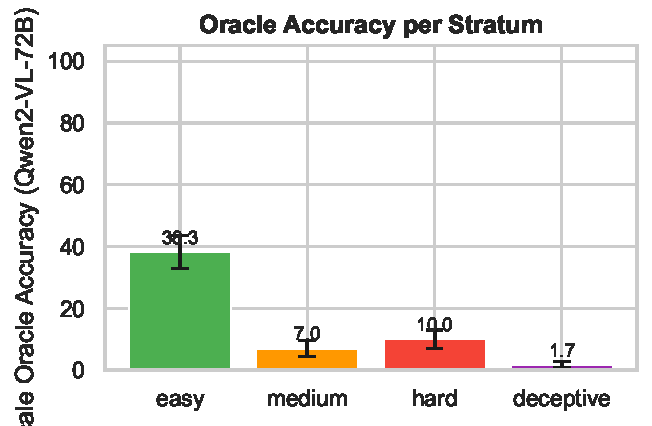
\includegraphics[width=\linewidth]{figures/fig4_oracle_validation.pdf}
  \caption{%
    \textbf{Qwen2-VL-72B accuracy per stratum (oracle validation, $n=455$).}
    Easy: 38.3\%; Medium: 7.0\%; Hard: 10.0\%; Deceptive: 1.7\%.  The
    Easy--Deceptive gap of \textbf{36.6}~pp is the strongest evidence that
    multi-model disagreement and unanimous-but-wrong consensus both reflect
    genuine difficulty rather than ensemble-specific idiosyncrasies.}
  \label{fig:oracle}
\end{figure}

\Cref{fig:oracle} shows Qwen2-VL-72B accuracy per stratum.
Easy: \textbf{38.3\%}; Medium: \textbf{7.0\%}; Hard: \textbf{10.0\%};
Deceptive: \textbf{1.7\%} (3 of 174 items).  The Easy--Hard gap is
\textbf{28.3}~pp and the Easy--Deceptive gap is \textbf{36.6}~pp,
both well above our 15~pp validity threshold.  This confirms that
multi-model disagreement is not a spurious signal but correlates with
genuine task difficulty as measured by an independent, stronger oracle.
(The 3~pp Hard--Medium difference is not statistically significant,
$\chi^2=0.26$, $p=0.61$.)

\paragraph{Deceptive is the hardest stratum for the oracle.}
The 72B oracle solves only 1.7\% of Deceptive items (95\% CI [0.0\%, 3.7\%]),
substantially below even the Hard stratum.  Per source: 0/138 VQAv2,
0/21 ChartQA, 0/3 TextVQA, 3/12 RealWorldQA.  The VQAv2 zero is partly a
verbosity artefact; the ChartQA zero is genuine---a same-family 72B model
also fails the chart questions that confuse all four 7B members,
supporting the Deceptive stratum as a window onto pretraining-level
blind spots.  Because all 81 Easy items come from RealWorldQA, the Easy
oracle accuracy (38.3\%) and the Easy--Hard gap also pick up a
source-dataset shift (see Limitations).

\subsection{Disagreement by Question Type}
\label{sec:qtypes}

\begin{figure}[t]
  \centering
  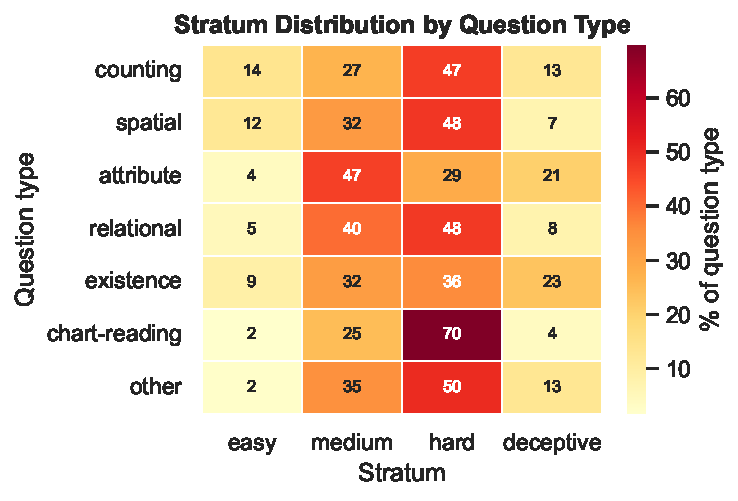
\includegraphics[width=\linewidth]{figures/fig3_heatmap.pdf}
  \caption{%
    \textbf{Stratum $\times$ question type.}
    Chart-reading and counting questions are disproportionately Hard;
    attribute questions are the least hard.}
  \label{fig:heatmap}
\end{figure}

\Cref{fig:heatmap} shows the stratum distribution across seven question types
(counting, spatial, attribute, relational, existence, chart-reading, and other).
Chart-reading and counting questions have the highest Hard fractions
(\textbf{69.7\%} and \textbf{47.0\%}), consistent with prior work showing
that enumerative and quantitative visual reasoning challenges current VLMs
disproportionately~\cite{tong2024mmvp,masry2022chartqa}.  Attribute
questions are the least hard (Hard fraction 28.8\%), suggesting that coarse
visual attribute detection (\eg colour, shape) is more reliably solved at 7B
scale.
The chi-square test for association between stratum and question type is
highly significant ($\chi^2 = 123.2$, $p < 0.001$, $df = 18$).

% ============================================================
\section{Discussion, Release, and Conclusion}
\label{sec:conclusion}

Multi-model disagreement is a cheap, robust signal of VQA difficulty:
four open-source 7B VLMs stratify 1{,}500 samples into informative
buckets validated by a 72B same-family oracle, at zero annotation cost.
Re-evaluating models on the Hard stratum alone would roughly halve
evaluation compute while providing \emph{more} discriminative signal;
we advocate routine stratum-stratified reporting over aggregate accuracy.
The Deceptive stratum---which the 72B oracle solves at only
1.7\%---is the most diagnostic of shared pretraining-level failures
and warrants mining for label auditing.
We release \dname{}, a 456-sample stratified subset (up to 125 per stratum,
Easy capped at 81) including the source image, question, ground truth, four
ensemble predictions, disagreement score, stratum label, and 72B oracle
result for the validated 455-item subset.
Dataset: \href{https://huggingface.co/datasets/AshwinP10/VQA-Disagree}{\nolinkurl{huggingface.co/datasets/AshwinP10/VQA-Disagree}}; code: \href{https://github.com/AshwinP10/vqa-disagree}{\nolinkurl{github.com/AshwinP10/vqa-disagree}}.

\paragraph{Limitations.}
All 81 Easy items come from RealWorldQA, so the 28.3~pp Easy--Hard oracle
gap partly reflects a source-dataset shift.  Our 7B ensemble may share
failure modes invisible at frontier scale, and the rule-based classifier
assigns 50.9\% of samples to ``other,'' limiting question-type resolution.

{\small
\bibliographystyle{ieeenat_fullname}
\bibliography{refs}
}

\end{document}
